\chapter{Red Neuronal}

\section{Planificación}
\subsection{Elección de framework y librerías}
En esta sección se defenderá la elección de las herramientas utilizadas
para el desarrollo de la red neuronal, resultando una ampliación de la
\textit{sección \ref{fwDL}}, donde se ha tratado más la materia en términos
del modelo apartándonos de su integración en el microcontrolador.

\textit{TensorFlow Lite} se utilizará para la creación del modelo optimizado
para microcontroladores, pero esto no perturba en absoluto el desarrollo
ordinario en \textit{TensorFlow}. Es decir, se trabajará de igual forma
que si la red neuronal se utilizara en un equipo convencional, con la
única salvedad de la conversión del modelo ya generado a una versión optimizada
para microcontroladores; así es la dinámica de trabajo con \textit{TinyML}.

Como complemento a \textit{TensorFlow} y para facilitar el desarrollo de la
red neuronal, se empleará \textit{Keras}, una \textit{API} de alto nivel
que, desde hace unos años, pertenece a \textit{TensorFlow}; sirviendo para
actuar como interfaz a nivel de capa para \textit{TensorFlow}, o expuesto de
otra forma, facilita el desarrollo al simplificar el trabajo con las capas
del modelo. Además también se utilizará para el estudio de los resultados
del entrenamiento.

Como entorno de desarrollo, se utilizará \textit{Google Colab}, se podrían
emplear alternativas que se ejecutan localmente como \textit{PyCharm},
\textit{Jupyter} o \textit{Eclipse}; sin embargo con \textit{Google Colab}
podemos aprovechar la capacidad de cómputo de sus \textit{GPU}s, lo cual agiliza
mucho los tiempos de \textit{entrenamiento} y \textit{validación}. Si bien,
el tiempo de uso del que se dispone de estas \textit{GPU}s, es limitado, aunque
siempre podemos continuar haciendo uso de las \textit{CPU}s. Además, al tratarse
de una alternativa en la nube, la etapa de configuración es mínima: apenas
instalando las librerías de las que vamos a hacer uso, ya tenemos desplegado
el entorno de trabajo.


\subsection{Diseño de la red neuronal}
El diseño de un modelo es determinante para que se desenvuelva apropiadamente
a la hora de realizar su función. Por más que se dote al modelo durante el
entrenamiento de un gran volumen de datos, será vano si el diseño no está enfocado
a la labor que tiene que desempeñar. Por lo tanto, para el diseño de este modelo,
se han estudiado otros muchos de clasificación de formas y procesamiento de imagen; la
mayoría hacían uso del célebre \textit{MNIST}: una base de datos que cuenta con
60.000 imágenes de entrenamiento y 10.000 de testeo, es un gran dataset de imágenes
de dígitos. Aunque en general se han consultado todo tipo de modelos para el
procesamiento de imágenes y clasificación, destacando el referente de este proyecto
\textit{Magic Wand}\textsuperscript{\cite{petewardenmw}} de \textit{Pete Warden}.
Para examinar con mayor profundidad la experimentación respecto al diseño del modelo,
observese el \textit{apéndice \ref{expRN}}.

El modelo que mejor funciona y más se utiliza en trabajos simples de procesamiento
de imagen para clasificación, es el de \textit{redes neuronales convolucionales}
(\textit{CNN}); definidas en una estructura muy marcada como ya se describió
en la Figura \ref{cnn}.
\begin{teoria}{Redes neuronales convolucionales}
Estas \textit{redes neuronales convolucionales}
no son más que un tipo de red neuronal que, reduciendo a un nivel muy básico,
utiliza un tipo de capa que realiza una operación matemática llamada convolución.

Lo cual nos lleva al siguiente paso, la definición de convolución: operador
matemático que haciendo uso de dos funciones $f$ y $g$, genera una nueva
a partir de estas, que representa la magnitud de su superposición.
Concretamente en 2 dimensiones, podemos entenderlo, tal y como ilustra la
Figura \ref{conv2d} como el producto del \textit{kernel} o \textit{filtro}
y una subventana de la matriz, generalmente una imagen; al repetir este producto
para todas las subventanas, obtenemos una nueva matriz resultado de la convolución.

Encontrar los valores del \textit{kernel} y por tanto la magnitud resultante
del análisis de la imagen de entrada, será la principal labor de la capa de
convolución.

Al resultado de la convolución, se le denomina \textit{mapa de características},
y su función es evidenciar dónde se encuentra la característica buscada por el
\textit{kernel}. Estos \textit{mapas de características} pueden reflejar
cambios de contraste, texturas, superficies planas, etc.

Pues bien, la red neuronal realizará esta operación secuencialmente, es decir,
el resultado de una capa, alimentará a la siguiente. Lo cual provoca que,
unido a un proceso de \textit{agrupación}, cada vez la información relevante
se condense y refine más y más, permitiendo extraer patrones cada vez más
complejos.
\end{teoria}\newpage

\begin{figure}[h]
    \centering
    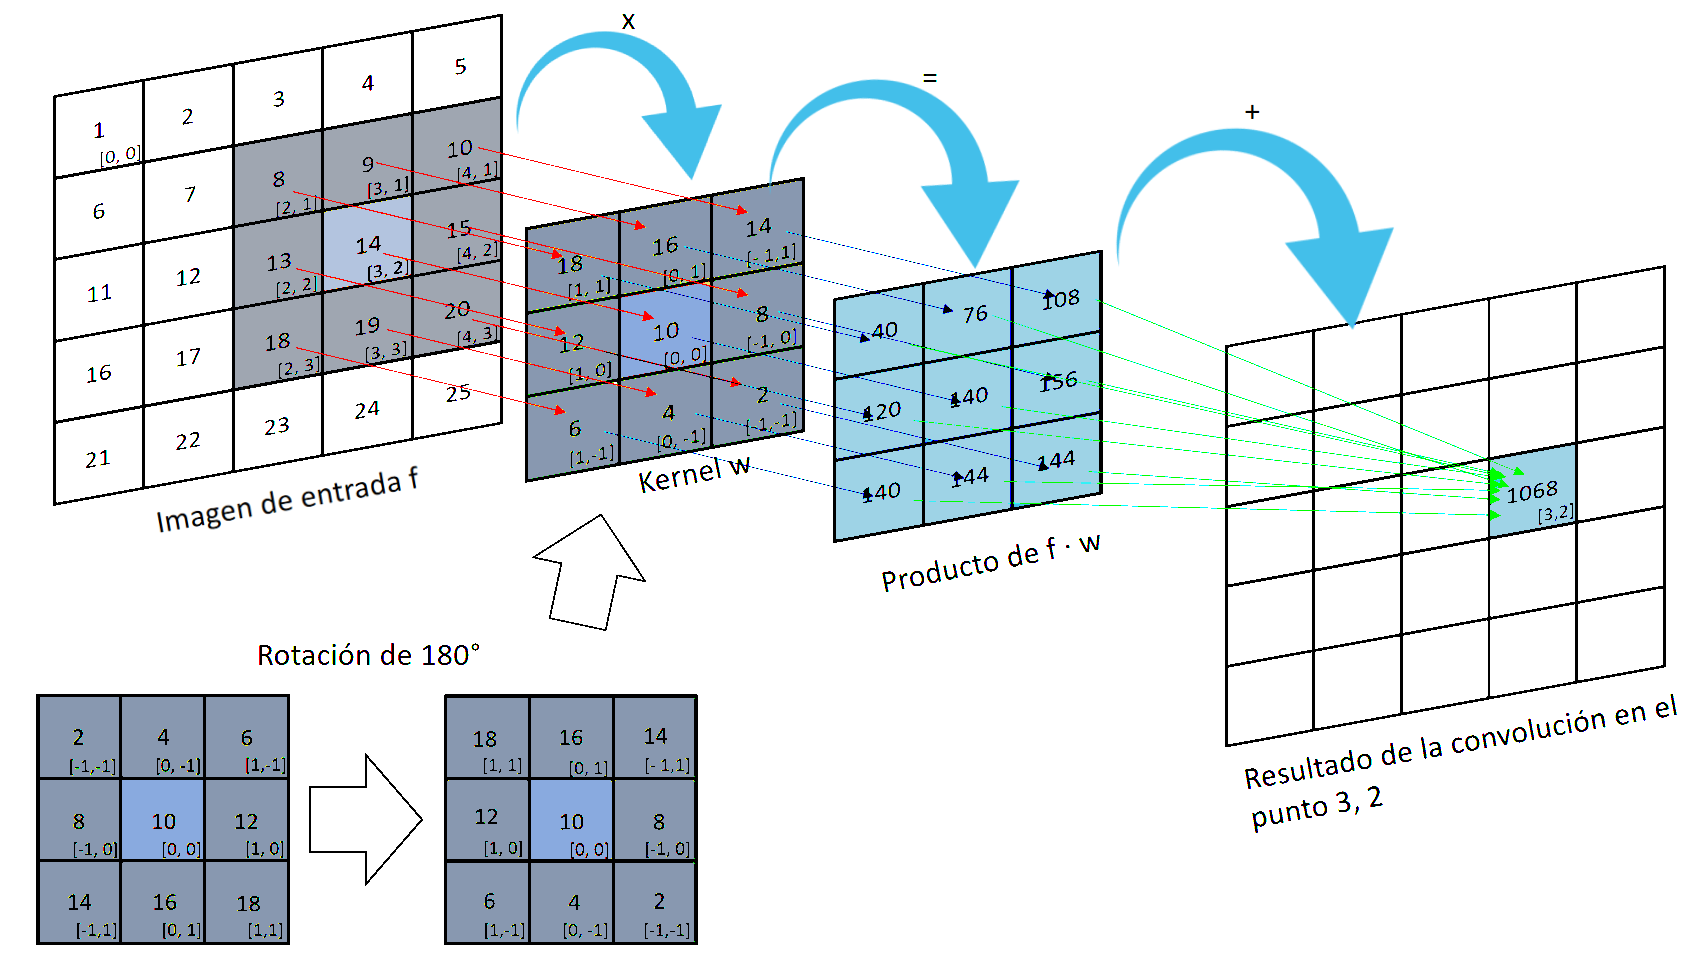
\includegraphics[width=1\textwidth]{capturas/conv2D.png}\\[-0,40cm]
    \caption{Esquema de convolución 2D\label{conv2d}
    {\scriptsize (\url{https://bryanmed.github.io/conv2d/})}}
\end{figure}

Conociendo la teoría de la \textit{red neuronal convolucional}, 
ya es posible comentar el diseño concreto implementado.
El modelo cuenta con una estructura de
\textit{Sequential} de \textit{Keras};
gracias a esta utilidad, es posible añadir capas al modelo de forma cómoda, además
de permitir el acceso a algunas funciones para el entrenamiento.
Se describirá la estructura en términos generales, para encontrar una descripción
a nivel de implementación real con \textit{Keras}, véase el \textit{apéndice
\ref{capasKeras}}

El modelo utilizado va a contar con tres bloques de procesamiento tras la entrada,
formados por una capa de \textit{convolución}, otra de \textit{normalización}, \textit{activación} y \textit{fropout}.
Estos bloques deben su composición a que el aporte de cada una de las capas,
complementa al procesamiento convolucional, en el caso de nuestro modelo, que
trabaja con imágenes tan pequeñas, son prácticamente irremplazables.
Comenzando por la inherente capa de \textit{convolución}, donde se dará el
procesamiento anteriormente ilustrado. Tras esta, se normaliza la salida mediante una capa
para este propósito, lo cual garantiza una mayor estabilidad y eficiencia
en el proceso de aprendizaje. Se define como función de activación, \textit{relu}; no
por otra cosa que porque es la más utilizada, la que mejor funciona para prácticamente
todas las labores sin tener que profundizar en el estudio del mismo y por su bajo
coste computacional; destacable debido a la naturaleza del dispositivo en el que
se ejecutará la red neuronal. Y por último la capa de \textit{Dropout} para mitigar
el overfitting, un problema que se ha podido experimentar debido a que es una red
neuronal de reducida complejidad.

En cada uno de los tres bloques, lo único que varía es el número de filtros de
la capa de convolución, duplicándose respecto al anterior.

Comentada la estructuración de estos bloques y su fundamento, ya es posible
desarrollar el modelo completo.
Al inicio, preliminar a los tres bloques citados, hay una capa de \textit{reescalado},
que va a servir meramente para normalizar los valores los píxeles de las imágenes
a una escala [0,1].
Tras esta, se encuentran los tres bloques descritos y posterior a estos,
una capa de \textit{agrupación} por simple
coherencia estructural debido a que reduce la dimensionalidad pero conserva la mayor
parte de información relevante (utilizada en la práctica totalidad de \textit{CNN}s).
Otra capa \textit{dropout} por el mismo motivo que en los
bloques y finalmente una capa densa \textit{softmax} con la que obtendremos una distribución
de probabilidad y así adquirir un output clasificatorio del mismo tamaño que número de letras
reconoce la red neuronal. Toda esta arquitectura se ilustra, simplificada, en la Figura \ref{esqRN}.

\begin{figure}[h]
    \centering
    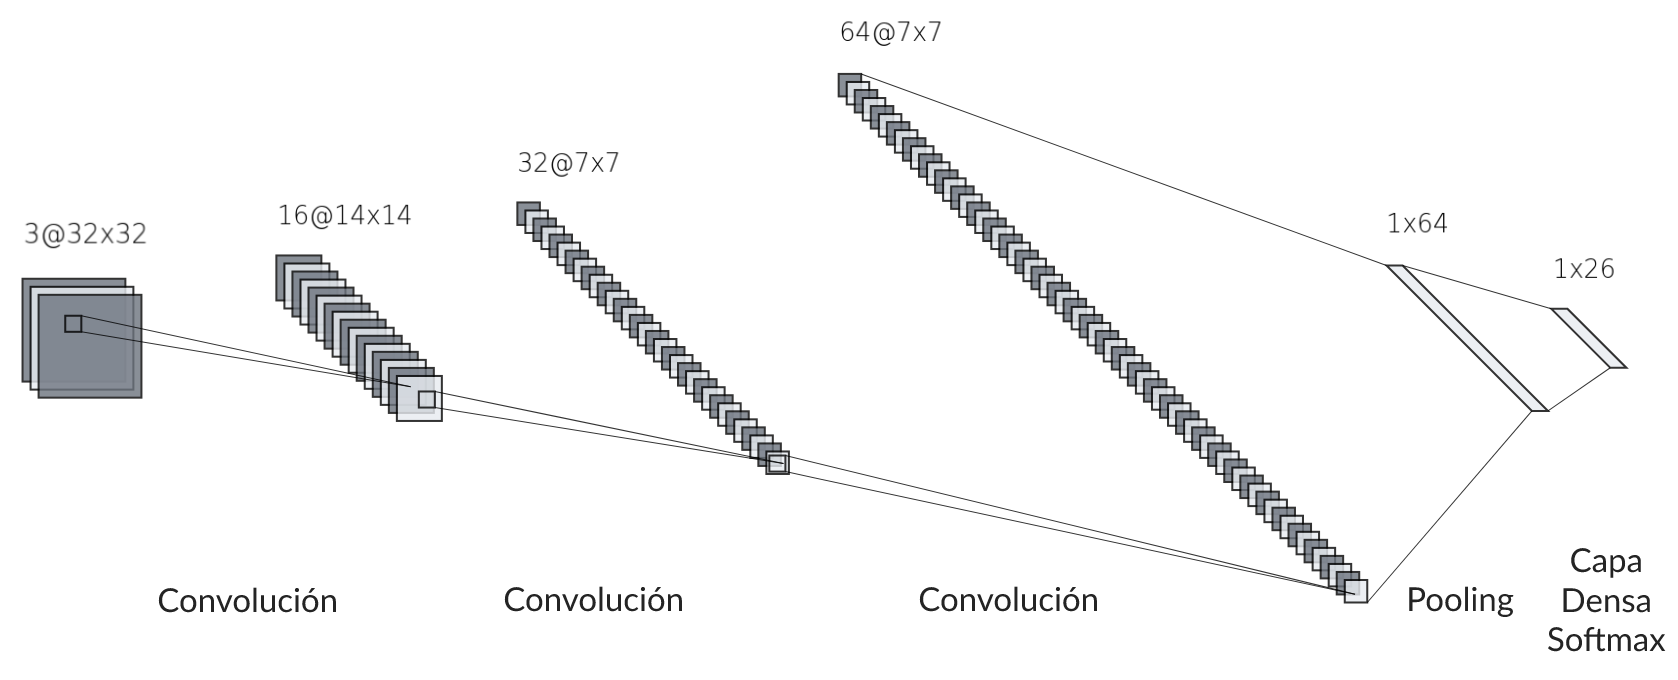
\includegraphics[width=1\textwidth]{capturas/esquemaRN.png}\\[-0,40cm]
    \caption{Esquema de la red neuronal diseñada \label{esqRN}}
\end{figure}

\section{Implementación}
\subsection{Preparativos}
Previo al diseño, se han de instalar ciertas dependencias y definir
algunos parámetros asistentes para el código. La mayoría de dependencias
son para trabajar con estructuras de datos en python, interfaces con el OS, o
librerías para \textit{TensorFlow} y \textit{Keras}.
También se ha hecho uso de algunas funciones del trabajo de
\textit{Pete Warden}\textsuperscript{\cite{petewardenmw}}.

Otra dependencia imprescindible es \textit{xxd}.
\begin{teoria}{Uso de \textit{xxd}\textsuperscript{\cite{tf-xxd}}}
    \color{mitexto}
    Es esencial contar con \textit{xxd}, esto se debe a que la mayoría de
    microcontroladores no tienen soporte para sistema de archivos nativo.
    Con \textit{xxd} obtenemos el modelo en formato matriz de chars directamente
    compatible con \textbf{C/C++} e integrable en cualquier microcontrolador.\newline
    Es recomendable establecer esta matriz como constante por cuestiones de
    eficiencia en el acceso a memoria.
\end{teoria}
\newpage

También necesitaremos el dataset para el entrenamiento, validación y testeo
del modelo. Se ha decidido que en pos de la experimentación y de un mejor desempeño
de la red neuronal al entrenarla con muestras generadas de la misma forma que se generarán
las que se procesen cuando se haga uso de esta en el microcontrolador; que se generarán
las muestras que utilizaremos como dataset, es decir, se va a generar un dataset propio.
Este datase se irá
actualizando a medida que se toman más muestras y que se podrá descargar
desde el \textit{Google Drive} institucional. Se acompaña la descarga de una comprobación
de existencia del fichero descargado para concluir esta sección.

Con el dataset descargado, se almacenan los trazos en un array, en el que
cada elemento del array será un trazo; de momento de todos los labels.

Los trazos en este momento están cargados como conjunto de coordenadas que
conforman, unas seguidas de otras, un recorrido; presumiblemente una letra.
Pero como ya es sabido, nuestro modelo necesita como entrada imágenes; por lo que
el siguiente paso es rasterizar los trazos para producir una imagen.

Al igual que en el firmware del microcontrolador, se hará uso de la función de rasterización creada
por \textit{Pete Warden}\textsuperscript{\cite{petewardenmw}}. Definidas las funciones de
rasterización, es posible rasterizar todos los trazos del dataset y destinarlos a las distintas
fases del desarrollo del modelo como se verá en las siguientes secciones.

{\color{red}Hablar de bloque 'PREPARE DATASETS'}

\subsection{Entrenamiento}
El entrenamiento del modelo será el segundo puntal que, junto con el diseño del
propio modelo, dotará de estabilidad a nuestra red neuronal; siendo ambas dos
determinantes para que esta responda de forma óptima a la tarea para la que a
la que ha sido dispuesta.
Por lo que la configuración del entrenamiento debe ser lo mejor posible, ajustando
\textit{epochs} (iteraciones en el proceso de entrenamiento), \textit{learning\_rate}
(escalabilidad del aprendizaje), \textit{optimizadores}, etc.
Para ver el ajuste experimental de estos valores, véase el \textit{apéndice \ref{expRN}}.

Las imágenes de los datasets ocuparán 32x32 píxeles. Este es otro parámentro que puede
ser estudiado, no obstante, estas dimensiones han sido las que han arrojado mejores
resultados de forma homogénea. Como de costumbre, para más información a este respecto,
consultar el \textit{apéndice \ref{expTrainRN}}.

Se utilizará el mismo conjunto de datos aleatoriamente distribuido para cada
uno de los tres dataset. Cada dataset contará con un porcentaje del conjunto de datos
total. Estos porcentajes han sido estudiados y a priori no suponen extrema relevancia
más allá de que el de entrenamiento debe ser ampliamente mayor. Ha sido fijado un
10\% para test, otro 10\% para validación y el restante 80\% para entrenamiento.
\newpage
\begin{teoria}{Uso del dataset en \textit{Deep Learing}(1)\textsuperscript{\cite{Andreas}}}
    \color{mitexto}
    Los tres datasets que se usan para \textit{Deep Learing} son:
    \begin{itemize}
        \itemsep0em
        \item \textbf{Validation}\\
        {\small En \textit{Deep Learning} se usan datos de validación para corroborar
        durante el entrenamiento, que el ajuste se está dando de forma óptima.\newline
        Dilatando un poco más esta sencilla explicación, el \textit{validation dataset}
        es un conjunto de datos imperativamente distinto del \textit{training dataset},
        que sirve para estimar la eficacia de la red en tiempo de entrenamiento.\newline
        En general se suele usar la validación para hacer estudios del ajuste del modelo,
        para evitar sobreajustes (\textit{overfitting}) y subajustes (\textit{underfitting}).}
        \begin{teoria}{\textit{Overfitting} y \textit{Underfitting}\label{ovYun}}
            \color{mitexto}
            \begin{itemize}
                \item \textbf{\textit{Overfitting}}\\
                {\small Es un fenómeno que se da cuando el modelo reconoce peculiaridades
                demasiado específicas como distintivo para la evaluación. Estas
                peculiaridades no serían los rasgos o características que constituyen
                a los elementos que estudiados y por lo tanto se produce un
                sobreajuste; un ajuste por encima de lo óptimo.} 
                \item \textbf{\textit{Underfitting}}\\
                {\small Término análogo y opuesto al anterior, el ajuste se
                presentaría laxo y falto de rigurosidad; ajuste por debajo de
                lo óptimo.} 
            \end{itemize}\end{teoria}
        \item \textbf{Training}\\
        {\small Este dataset es el más simple de entender por mera inmediación
        semántica. Es el conjunto de datos que se utiliza en tiempo de entrenamiento
        para balancear los pesos de las capas. En cada iteración de entrenamiento,
        se calcula la pérdida con los datos de entrenamiento introducidos y
        se da el ajuste de pesos en base a la pérdida. Esto supone que, cada vez la
        pérdida sea menor y generalmente la eficacia, o en términos más comunes a este
        ámbito, la \textit{precisión} (\textit{accuracy}), sea mayor.}
        \item \textbf{Test}\\
        {\small El conjunto de datos que se utilizará posterior al entrenamiento, para
        validar la efectividad del entrenamiento.
        Es el dataset con el que se pone a prueba el modelo entrenado.}
    \end{itemize}
\end{teoria}
\newpage

\subsection{Testeo}
El testeo del modelo es útil para garantizar que funciona correctamente, sin
embargo podemos obtener valores muy buenos sin resultar en un funcionamiento
adecuado, debido al ya mencionado \textit{overfitting} (\textit{Teoría \ref{ovYun}}).
Por tanto solo debemos tomarlo como una herramienta más, siempre evaluando
adecuadamente los resultados.

La fase de testeo consiste en simular lo que será una ejecución habitual,
pero conociendo los inputs de la red neuronal, que serán del dataset
de testeo. Obteniendo imágenes de cada letra (\textit{label}), se evalúa
la clasificación de la red neuronal de la misma, junto con la precisión
de estimación; si la clasficación coincide y además lo hace con valores de
precisión próximos a 1, significará, en principio, un buen desempeño de la red
neuronal para
esta letra. El objetivo es conseguir esto para todas las letras.

Es importante separar los dataset de testeo de los de entrenamiento
y validación, ya que si se emplearan los mismos, el modelo ha sido entrenado
con este mismo input, por tanto siempre se obtendrían buenos resultados
y el testeo perdería validez.

Para un mayor acercamiento a la experimentación con el testeo de los modelos
probados, visite el \textit{apéndice \ref{expTrainRN}}

\subsection{Transformación a modelo cuantizado}
El hecho de cuantizar el modelo basado en \textit{Deep Learning} cuando se
plantea su integración en microcontroladores y equipos de bajo rendimiento,
suele ser imperativo.

\begin{teoria}{Cuantización}
    \color{mitexto}
    Cuantizar es desvirtuar la naturaleza continua de un conjunto de valores continuos,
    restringiéndolos a un conjunto de valores discretos.
\end{teoria}

En general esta práctica viene propiciada debido a que
la mayoría de microcontroladores no cuentan con \textit{FPU}
(\textit{Floating Point Unit}). Sin embargo no es este el caso, ya que en este
proyecto se escogió un microcontrolador que sí dispone de esta unidad. Aun
así se ha tenido que recurrir a la cuantización del modelo, como consecuencia
de su limitación de memoria, ya que el hecho de cuantizar el modelo, supone
reducir su precisión y por tanto reducir la memoria que este requiere.

Sin entrar en muchos detalles, ya que es parte de la siguiente sección,
el modelo generado estándar queda muy lejos de poder integrarse en el
microcontrolador, gracias a la conversión a un modelo \textit{TensorFlow Lite},
se reduce el tamaño, pero sigue sin ser suficiente, por tanto es conveniente
cuantizar el modelo \textit{TensorFlow Lite} para obtener su
versión más compacta posible.


\subsection{Comparación de modelos generados}
Los modelos generados para la red neuronal, se muestran en la Tabla \ref{tabModelos}.
\begin{table}[h]
    \color{mitexto}
    \begin{tabular}{llll}
    \rowcolor[HTML]{6C737E} 
    {\color[HTML]{EFEFEF} \textbf{Modelo}}     & {\color[HTML]{EFEFEF} \textbf{Tamaño}} & \cellcolor[HTML]{6C737E}{\color[HTML]{EFEFEF} \textbf{Reducción TF}} & \cellcolor[HTML]{6C737E}{\color[HTML]{EFEFEF} \textbf{Reducción TFLite}} \\
    \rowcolor[HTML]{CDDADE} 
    TensorFlow                                 & 756009 Bytes~~                           & \cellcolor[HTML]{CDDADE}0\%                                          & \cellcolor[HTML]{CDDADE}-                                                \\
    \rowcolor[HTML]{E8ECF1} 
    TensorFlow Lite                            & 140300 Bytes~~                           & \cellcolor[HTML]{E8ECF1}81'4\%                                       & \cellcolor[HTML]{E8ECF1}0\%                                              \\
    \rowcolor[HTML]{CDDADE} 
    \cellcolor[HTML]{CDDADE}TF Lite cuantizado & 41136 Bytes~~                            & 94'5\%                                                               & 70'6\%                                                                  
    \end{tabular}
    \caption{Tabla de comparación de modelos generados\label{tabModelos}}
\end{table}

Los resultados son impresionantes en sí mismos, pero lo son aún más cuando ponemos
en contexto los valores de precisión que se alcanzan para cada uno de ellos en
la clasificación; variando en el peor de los casos del orden de 0,1\% de
\textit{TensorFlow} a \textit{TensorFlow Lite} y del orden de 0,2\% de
\textit{TensorFlow} a \textit{TensorFlow Lite} cuantizado.
Por lo que la compactación del modelo no tiene un impacto notorio
durante su ejecución.

\subsection{Integración en el microcontrolador\label{RNenμC}}
Esta sección sirve ahora a modo de recopilación de las anteriores,
ya que el procedimiento prácticamente ha sido expuesto.

La cuantización del modelo para optimizar el uso de memoria es el primer
paso; una vez el modelo cuenta con un tamaño apto para el microcontrolador,
lo que resta es solucionar el problema de la carencia de sistema de archivos
necesario para el manejo de la red neuronal construida con \textit{TensorFlow}.
Para lo cual se hace uso de \textit{xxd}, herramienta que automatiza el proceso
de conversión del modelo a una estructura de datos (\textit{vector} de
\textit{chars}), agregable al firmware del microcontrolador.

Cuando pasamos el modelo por \textit{xxd} y obtenemos el código en \textit{C},
es suficiente con añadirlo al código del \textit{firmware} y este ya es funcional
en el microcontrolador. Con el que se trabajará gracias a las librerías de
\textit{TensorFlow Lite}.

\section{Generación de muestras para el dataset\label{dataColl}}
Por suerte se podremos contar con una herramienta creada por
\textit{Pete Warden}\textsuperscript{\cite{petewardenmw}} para tomar
muestras de trazados con el microcontrolador que estamos empleando.
Se ha modificado superficialmente y se han hecho algunos cambios
estéticos (\href{https://github.com/AntonioPriego/SmartPen/blob/main/DataCollector/SmartPen_DataCollector.html}{DataCollector.html}). 
Este proceso supone, para el sujeto que genera las muestras, un tiempo de
adaptación al movimiento que se debe ejecutar para que se recoja un buen trazado,
añadido al hecho de que las muestras que no sean óptimas, deben eliminarse;
lo convierten en un proceso cargante y lento para quien está creando las muestras
y para quien tiene que supervisarlas.

A lo largo de la toma de muestras se han detectado ciertos fallos que
se han resuelto y son consultables en los Apéndices \ref{PWchrome},
\ref{borrarMuestras} y \ref{borraIndices}.